\chapter{Collaboration between Nova controllers}
\label{sec:collaboration}



\section{Organisation of the collaboration between components of OpenStack}

Collaboration between components of OpenStack is based on three different ways:
AMQP \footnote{AMQP: Advanced Messaging Queuing Protocol} bus, HTTP APIs and
sharing of inner-states via a replicated relational databases. Each of the 
preceding way of collaborating have specific purposes: some are intended for 
local collaboration as with sub-services of a controller, while some of these
ways are intended for inter-controller collaboration.

\subsection{AMQP bus: making sub-services collaborating}

\subsection{HTTP APIs: making sub-services collaborating}

\subsection{Shared inner-states: collaboration between remote controllers}


\section{Creation of a VM: detailed workflow}

During the study of OpenStack components, it was noticable that a large part of
the collaboration that happend between controllers during the creation of a VM
\footnote{VM: Virtual machine} was done via the sharing of inner-states.

\begin{sidewaysfigure}[htbp]
        \centering
        %http://www.websequencediagrams.com/?lz=dGl0bGUgQ3JlYXRpb24gb2YgYSBWTQoKVXNlciAtPiArY29uZHVjdG9yLm1hbmFnZXIqXG5AZWNvbm9tZTE1OiBidWlsZF9pbnN0YW5jZSgpCgATHgBPBXNjaGVkdWxlci5maWx0ZXJfAAgJAE4PACAJX3J1bgBZDAAbJwCBOwdtcHV0ZQCBLRM3OiAASQ8KIyBCdWlsZCAAgUkICgAjGy0-AD4eXwCCCxEKICAAKiZyZXNzb3VyY2VfdHJhY2tlcgCBKA0AgmYIX2NsYWltKCkATAsAHRwtPi0AgW8dAEYIAH0pAIFgFmFsbG9jYXRlX25ldHdvcmsAgRsFAIFZIAAlBwCDDxYASQlmb3IAhF8MICAgIAAeGy0-ADAmbWFjX2FkZHJlc3MAC0pmaXhlZF9pcABmQXVwZGF0ZV9kbgB4JQCDRB4AgwsHX2luZm8AhGwgAIQPHQCFKSEAhEweX3ByZXBfYmxvY2tfZGV2aQCDRwcAhjA8c3Bhd24AhEYldmlydC5kcml2AIZHDwA2DAAOFi0AhiIgb2s&s=default
        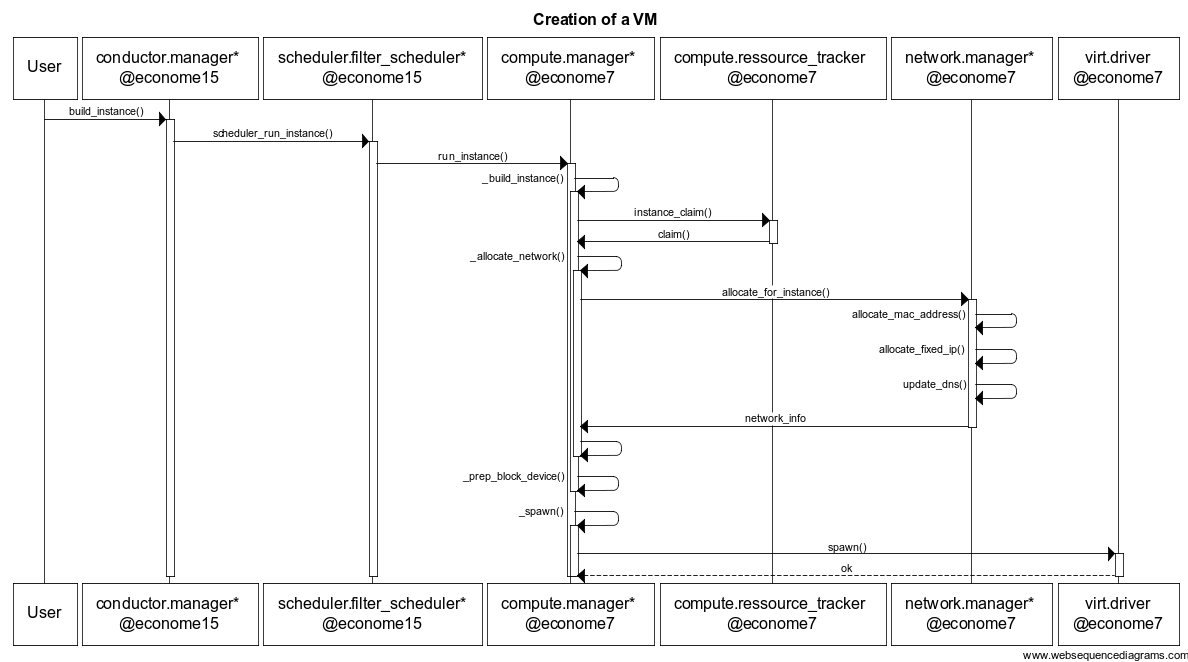
\includegraphics[width=23cm]{figures/sequence.png}        
        \caption{Services involved in the creation of a VM.}
        \label{fig:sequence_vm_creation}
\vspace*{-.3cm}
\end{sidewaysfigure}

Indeed, when a request for the creation of a VM was made, the \emph{nova-api}
sub-service performed actions that resulted in the storage of an VM object in
the database. A simplified view of this VM object can be found in the following
listing:

\begin{lstlisting}[language=json,firstnumber=1]
{
   'hostname':u'vm1',
   'vm_state':u'building',
   'progress':0,
   'project_id':u'1b46e91b72984e47ad0d8d127f59e978',
   'launched_at':None,
   'scheduled_at':None,
   'deleted':0,
   'key_name':None,
   'task_state':u'scheduling',
}
\end{lstlisting}

It is noticable that this object as